% Options for packages loaded elsewhere
\PassOptionsToPackage{unicode}{hyperref}
\PassOptionsToPackage{hyphens}{url}
\PassOptionsToPackage{dvipsnames,svgnames*,x11names*}{xcolor}
%
\documentclass[
  10pt,
  ignorenonframetext,
  aspectratio=43,
]{beamer}
\usepackage{pgfpages}
\setbeamertemplate{caption}[numbered]
\setbeamertemplate{caption label separator}{: }
\setbeamercolor{caption name}{fg=normal text.fg}
\beamertemplatenavigationsymbolsempty

%%
%%% Definition of colors
%%% Source: https://latexcolor.com/
\definecolor{blanchedalmond}{rgb}{1.0, 0.92, 0.8}
\definecolor{blond}{rgb}{0.98, 0.94, 0.75}
%%% End of definition of colors
%%

% Prevent slide breaks in the middle of a paragraph
\widowpenalties 1 10000
\raggedbottom
\usepackage{lmodern}
\usepackage{amssymb,amsmath}
\usepackage{ifxetex,ifluatex}
\ifnum 0\ifxetex 1\fi\ifluatex 1\fi=0 % if pdftex
  \usepackage[T1]{fontenc}
  \usepackage[utf8]{inputenc}
  \usepackage{textcomp} % provide euro and other symbols
\else % if luatex or xetex
  \usepackage{unicode-math}
  \defaultfontfeatures{Scale=MatchLowercase}
  \defaultfontfeatures[\rmfamily]{Ligatures=TeX,Scale=1}
  \setmainfont[]{SF Pro Display}
  \ifxetex
    \usepackage{xeCJK}
    \setCJKmainfont[ItalicFont=AR PL UKai TW]{AR UDJingXiHeiPU30}
  \fi
  \ifluatex
    \usepackage[]{luatexja-fontspec}
    \setmainjfont[ItalicFont=AR PL UKai TW]{AR UDJingXiHeiPU30}
  \fi
\fi
\usetheme[]{metropolis}
\usecolortheme{default}
\usefonttheme{serif} % use mainfont rather than sansfont for slide text
% Use upquote if available, for straight quotes in verbatim environments
\IfFileExists{upquote.sty}{\usepackage{upquote}}{}
\IfFileExists{microtype.sty}{% use microtype if available
  \usepackage[]{microtype}
  \UseMicrotypeSet[protrusion]{basicmath} % disable protrusion for tt fonts
}{}
\makeatletter
\@ifundefined{KOMAClassName}{% if non-KOMA class
  \IfFileExists{parskip.sty}{%
    \usepackage{parskip}
  }{% else
    \setlength{\parindent}{0pt}
    \setlength{\parskip}{6pt plus 2pt minus 1pt}}
}{% if KOMA class
  \KOMAoptions{parskip=half}}
\makeatother
\usepackage{xcolor}
\IfFileExists{xurl.sty}{\usepackage{xurl}}{} % add URL line breaks if available
\IfFileExists{bookmark.sty}{\usepackage{bookmark}}{\usepackage{hyperref}}
\hypersetup{
  pdftitle={Powerful Women: Does Exposure Reduce Bias? },
  pdfauthor={Yu-Hsin Ho},
  colorlinks=true,
  linkcolor=Maroon,
  filecolor=Maroon,
  citecolor=Blue,
  urlcolor=red,
  pdfcreator={LaTeX via pandoc}}
\urlstyle{same} % disable monospaced font for URLs
\newif\ifbibliography
\usepackage{listings}
\newcommand{\passthrough}[1]{#1}
\lstset{defaultdialect=sh}
\lstset{framexleftmargin=0mm, frame=trBL,backgroundcolor=\color{blanchedalmond!5},numbers=left,numberstyle=\scriptsize,basicstyle=\small}
\lstset{aboveskip=5mm,belowskip=5mm,xleftmargin=20pt,xrightmargin=5pt}
% \lstset{prebreak={\raisebox{0ex}[0ex][0ex]}}
% \lstset{postbreak={\raisebox{0ex}[0ex][0ex]\space}}
\lstset{breaklines=true,breakatwhitespace=true}
\usepackage{longtable,booktabs}
\usepackage{caption}
% Make caption package work with longtable
\makeatletter
\def\fnum@table{\tablename~\thetable}
\makeatother
\usepackage{graphicx,grffile}
\makeatletter
\def\maxwidth{\ifdim\Gin@nat@width>\linewidth\linewidth\else\Gin@nat@width\fi}
\def\maxheight{\ifdim\Gin@nat@height>\textheight\textheight\else\Gin@nat@height\fi}
\makeatother
% Scale images if necessary, so that they will not overflow the page
% margins by default, and it is still possible to overwrite the defaults
% using explicit options in \includegraphics[width, height, ...]{}
\setkeys{Gin}{width=\maxwidth,height=\maxheight,keepaspectratio}
% Set default figure placement to htbp
\makeatletter
\def\fps@figure{htbp}
\makeatother
\setlength{\emergencystretch}{3em} % prevent overfull lines
\providecommand{\tightlist}{%
  \setlength{\itemsep}{0pt}\setlength{\parskip}{0pt}}
\setcounter{secnumdepth}{-\maxdimen} % remove section numbering

%
% When using babel or polyglossia with biblatex, loading csquotes is recommended 
% to ensure that quoted texts are typeset according to the rules of your main language.
%
\usepackage{csquotes}

%
% blockquote
%
\definecolor{blockquote-border}{RGB}{221,221,221}
\definecolor{blockquote-text}{RGB}{89,89,89}
\usepackage{mdframed}
\newmdenv[rightline=false,bottomline=false,topline=false,linewidth=3pt,linecolor=blockquote-border,skipabove=\parskip]{customblockquote}
\renewenvironment{quote}{\begin{customblockquote}\list{}{\rightmargin=0em\leftmargin=0em}%
\item\relax\color{blockquote-text}\ignorespaces}{\unskip\unskip\endlist\end{customblockquote}}

%
% Source Sans Pro as the de­fault font fam­ily
% Source Code Pro for monospace text
%
% 'default' option sets the default 
% font family to Source Sans Pro, not \sfdefault.
%

\usepackage{adjustbox}
\usepackage{booktabs}
\linespread{1.3}
\usepackage[font={footnotesize}]{caption}

\title{Powerful Women: Does Exposure Reduce Bias? \footnote<.->{Beaman,
  L., Chattopadhyay, R., Duflo, E., Pande, R., \& Topalova, P. (2009).
  Quarterly Journal of Economics, 124(4), 1497-1540.}}
\subtitle{Applied Microeconomics \textbar{} 2022 Spring}
\author{Yu-Hsin Ho}
\date{May 23, 2022}
\institute{Department of Economics, National Taiwan University}

\begin{document}
\frame{\titlepage}

\hypertarget{introduction}{%
\section{Introduction}\label{introduction}}

\begin{frame}{Introduction}
General discussion around gender quota policy:

\begin{enumerate}
\tightlist
\item
  \textbf{Empathy/Information Provision}: exposure improves
  understanding, updating prior belief to reduce statistical
  discrimination
\item
  \textbf{Backlash}: ``reverse discrimination'', threatened status for
  privileged group
\end{enumerate}
\end{frame}

\begin{frame}{Identification: Female Quota in Indian Local Councils}
\protect\hypertarget{identification-female-quota-in-indian-local-councils}{}
\emph{Panchayat}: District \textgreater{} Block \textgreater{}
\textbf{Village} (\emph{Gram Panchayats, GP})

\begin{itemize}
\tightlist
\item
  1993 Constitutional Amendment

  \begin{itemize}
  \tightlist
  \item
    1/3 councilor seats reserved for female
  \item
    1/3 GPs' chief councilor (\emph{Pradhan}) reserved for female,
    chosen randomly.
  \end{itemize}
\end{itemize}

\begin{block}{Sample}
\protect\hypertarget{sample}{}
\begin{itemize}
\tightlist
\item
  Sample: GPs in West Bengal

  \begin{itemize}
  \tightlist
  \item
    Active elections long before the amendment.
  \end{itemize}
\item
  Electoral results from 1998, 2003, 2008
\item
  Supplemented by survey and experimental data
\end{itemize}
\end{block}
\end{frame}

\begin{frame}{Research Design}
\protect\hypertarget{research-design}{}
Exogenous Treatment: \textbf{Reservation}

\begin{itemize}
\tightlist
\item
  \(\xrightarrow{\text{(1) Election}}\) Electoral Outcomes: Current and
  prospect
\item
  \(\xrightarrow{\text{(2) Survey}}\) Evaluation of Female Leader's
  Effectiveness
\item
  \(\xrightarrow{\text{(3) Experiments}}\) Gender Bias \& Stereotype
\end{itemize}
\end{frame}

\begin{frame}
\begin{figure}
\centering
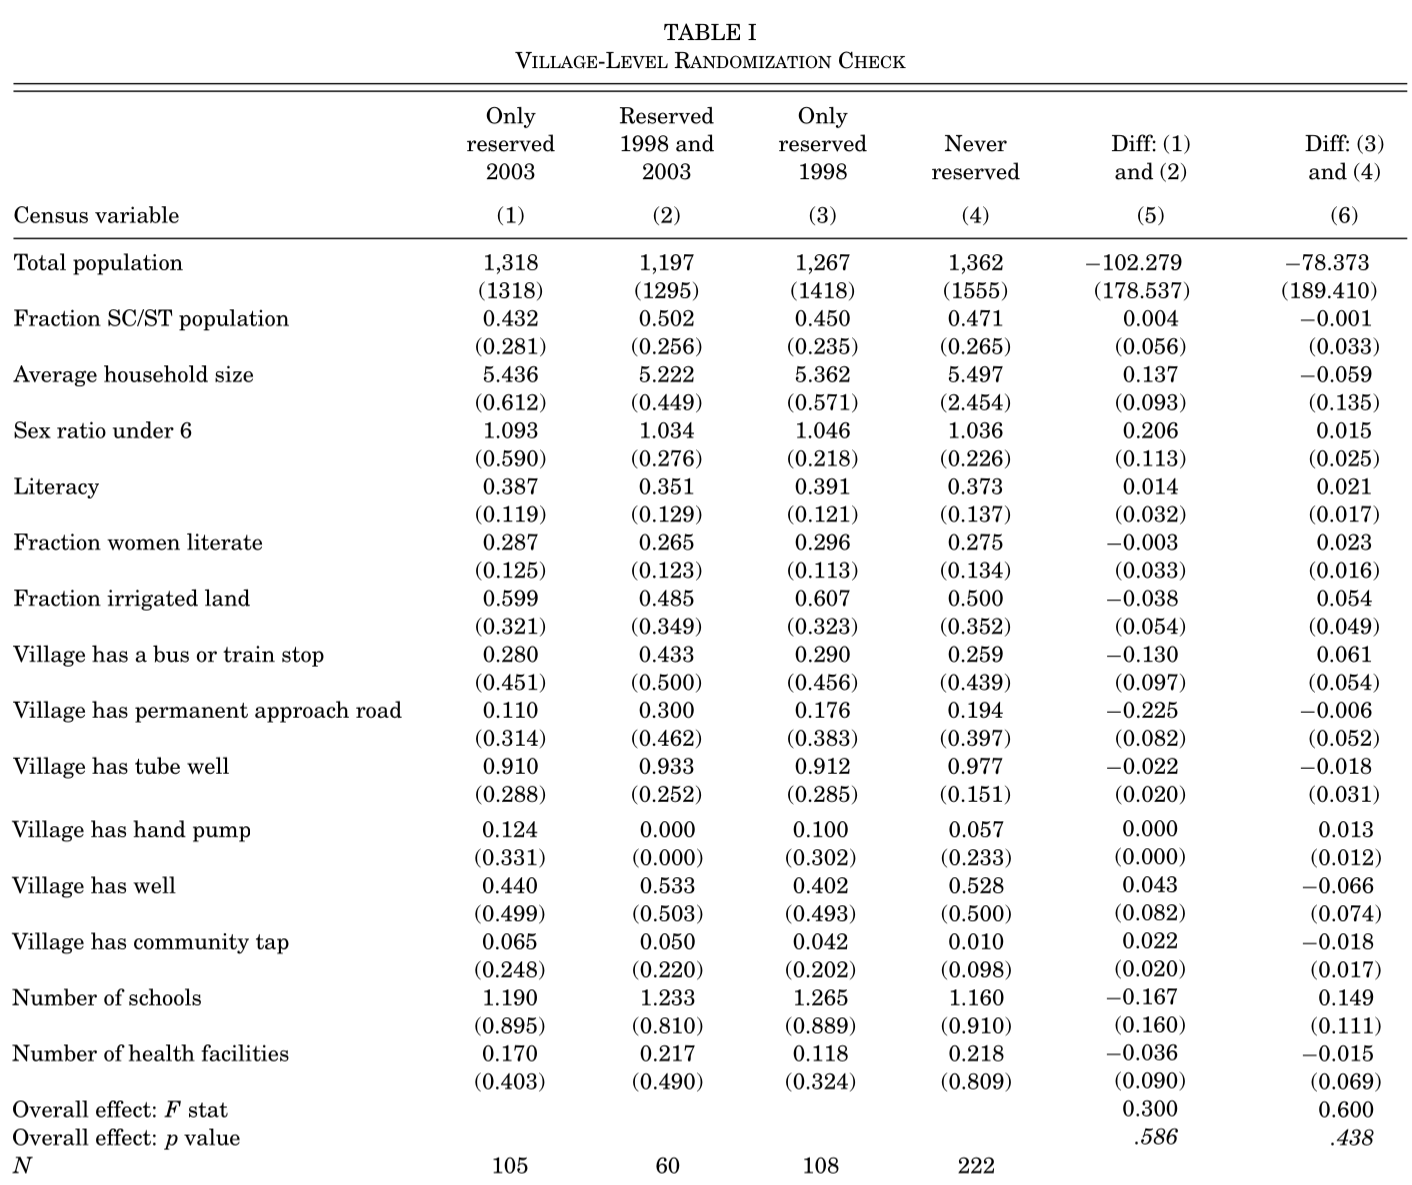
\includegraphics{20220523-qje-beaman-duflo-powerful-women.assets/table1-randomization-check.png}
\caption{Randomization Check}
\end{figure}
\end{frame}

\hypertarget{outcome-electoral-results}{%
\section{Outcome: Electoral Results}\label{outcome-electoral-results}}

\begin{frame}{Short-term: Reservation is Binding}
\protect\hypertarget{short-term-reservation-is-binding}{}
\begin{figure}
\centering
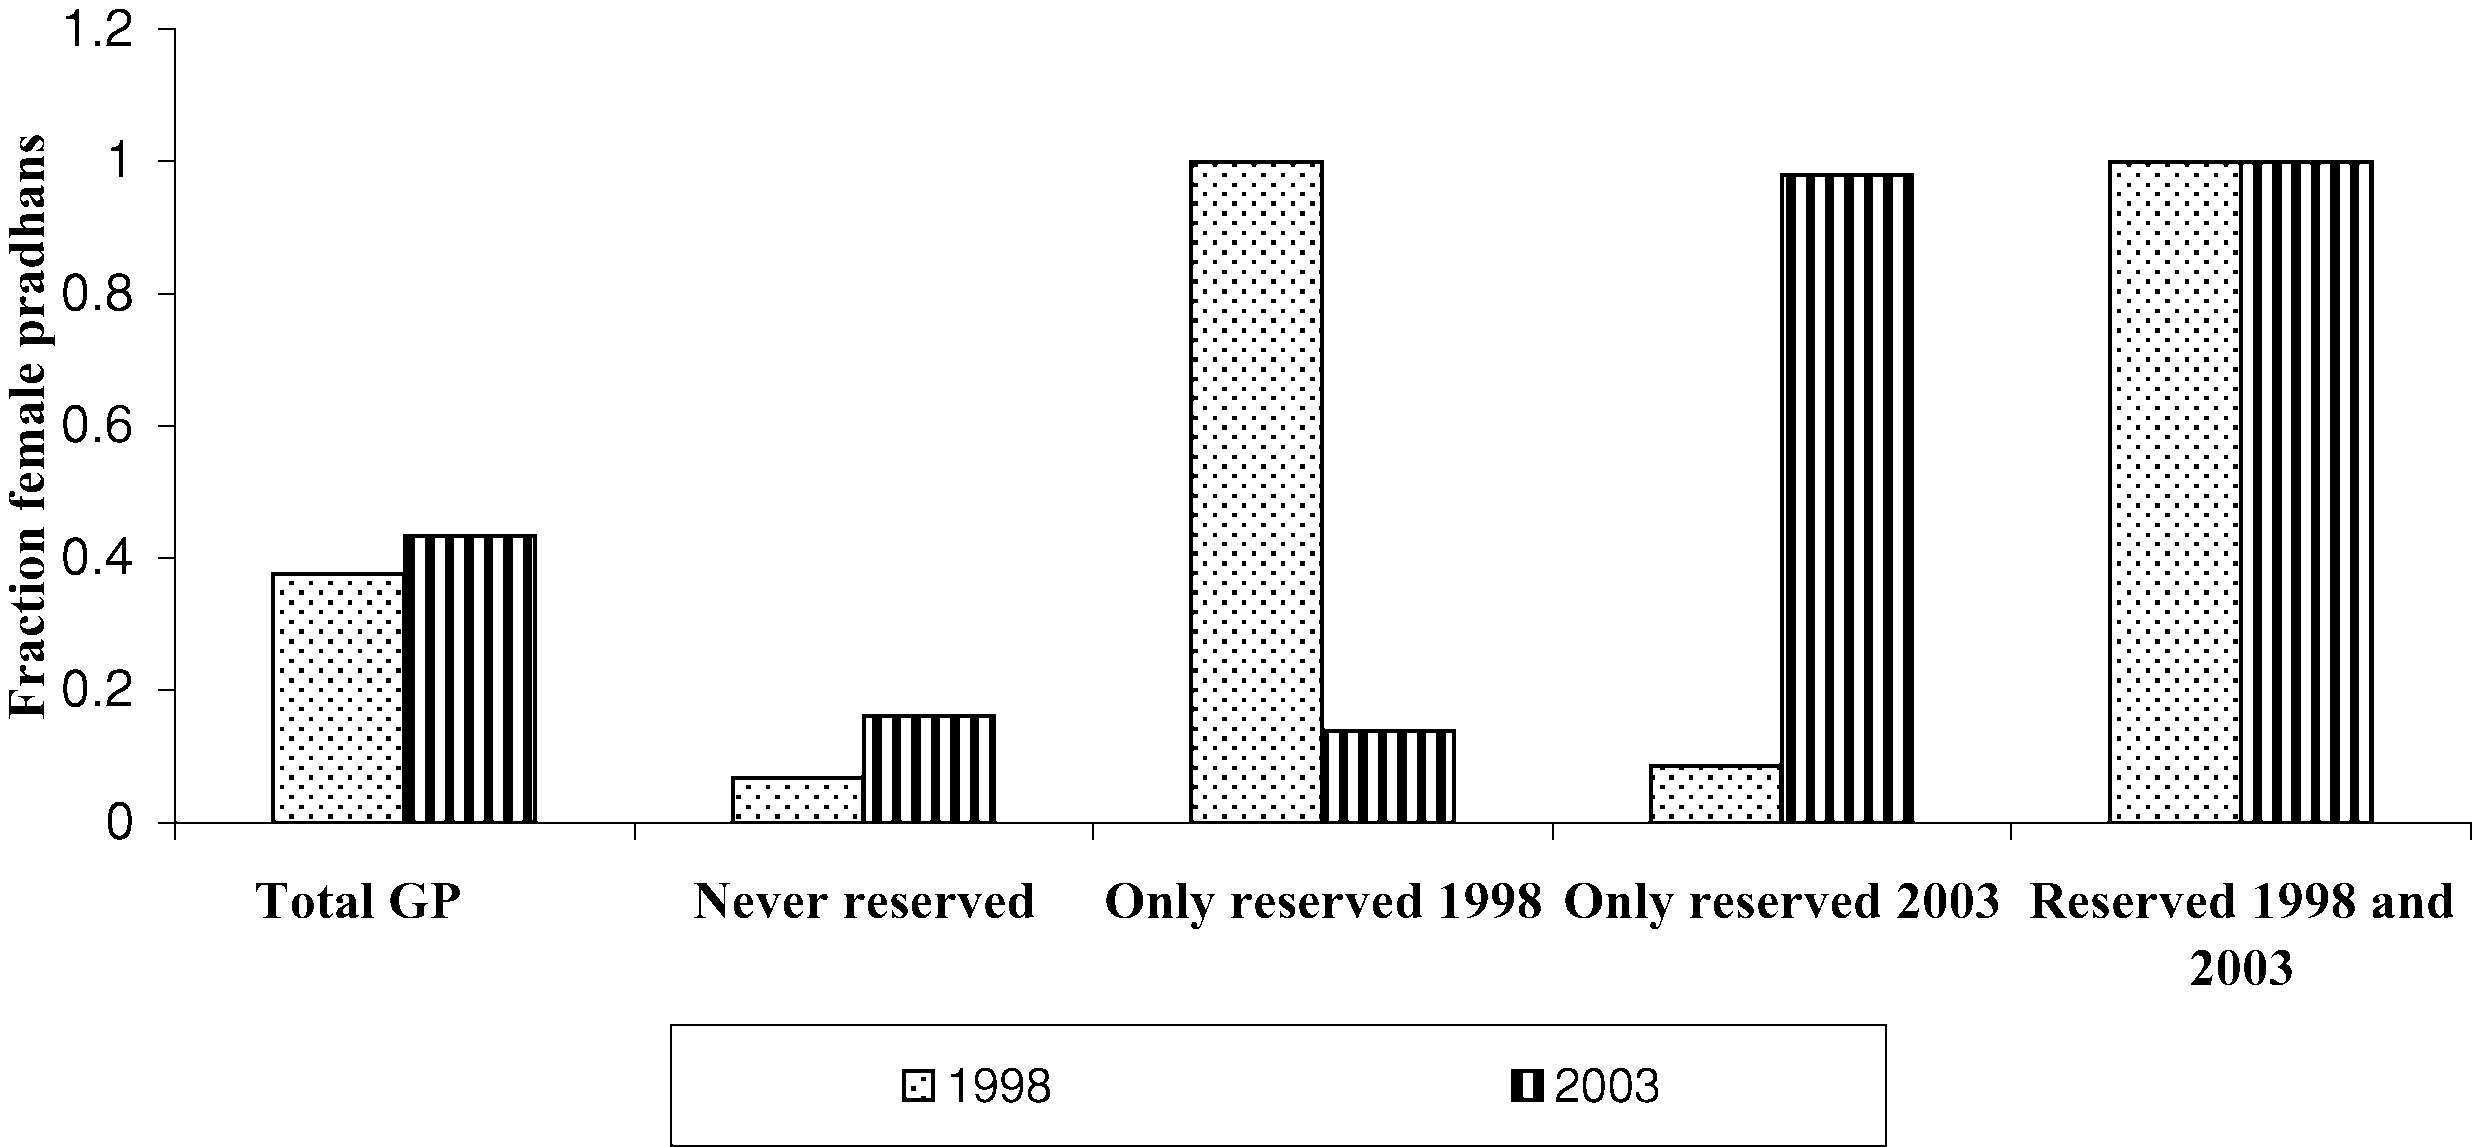
\includegraphics{20220523-qje-beaman-duflo-powerful-women.assets/figure1-binding policy effect.png}
\caption{Fraction of Female Pradhan by Reservation Status}
\end{figure}
\end{frame}

\begin{frame}{Long-term: Improved Female Electoral Prospect}
\protect\hypertarget{long-term-improved-female-electoral-prospect}{}
\begin{figure}
\centering
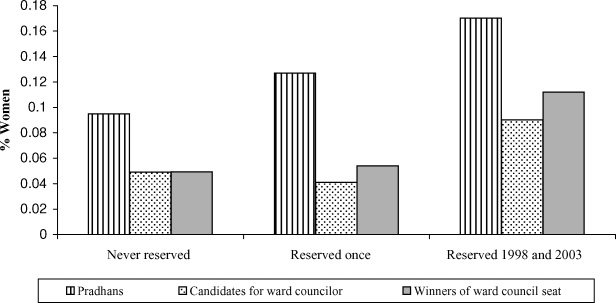
\includegraphics{20220523-qje-beaman-duflo-powerful-women.assets/figure2-electoral prospect.png}
\caption{2008 Ward Council and Pradhan Election Outcomes}
\end{figure}
\end{frame}

\begin{frame}
\begin{figure}
\centering
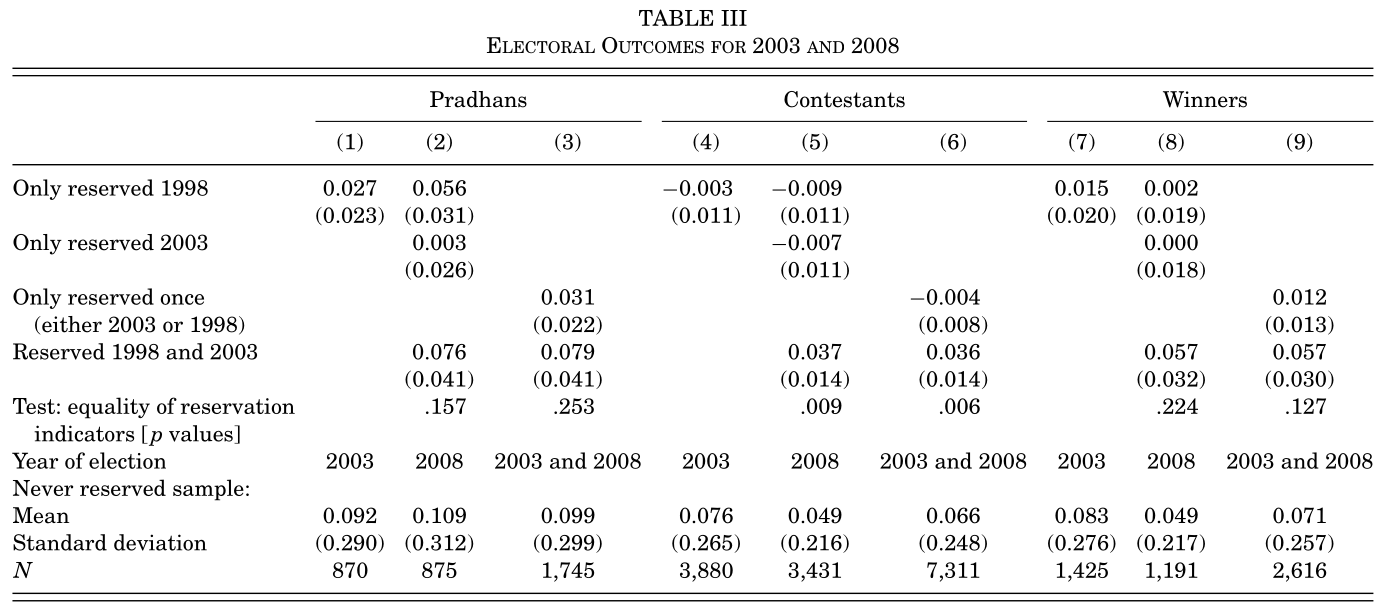
\includegraphics{20220523-qje-beaman-duflo-powerful-women.assets/table3-electoral outcomes.png}
\caption{Electoral Outcomes for 2003 and 2008}
\end{figure}
\end{frame}

\hypertarget{survey-evaluation-of-pradhan}{%
\section{Survey: Evaluation of
Pradhan}\label{survey-evaluation-of-pradhan}}

\begin{frame}{Survey: Evaluation of Pradhan}
\begin{itemize}
\tightlist
\item
  Survey: 2006-2007 (in-office pradhan elected in 2003)
\item
  495 villages, 165 GPs in Birbhum District, West Bengal
\item
  15 households per village
\item
  Questions

  \begin{enumerate}
  \tightlist
  \item
    ``Is pradhan effective''
  \item
    ``Did pradhan look after village needs''
  \item
    ``Did pradhan look after your needs''
  \item
    ``Did pradhan make BPL\footnote<.->{Below poverty line} lists well''
  \end{enumerate}
\end{itemize}
\end{frame}

\begin{frame}
\begin{figure}
\centering
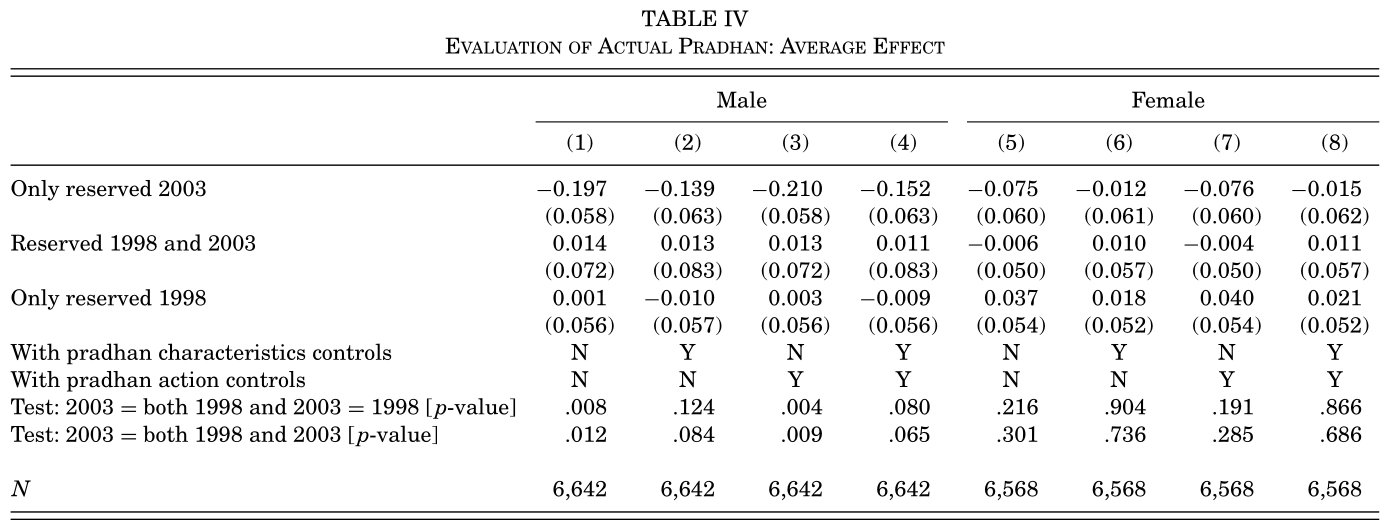
\includegraphics{20220523-qje-beaman-duflo-powerful-women.assets/table4-evaluation of pradhan.png}
\caption{Evaluation of 2003-elected Pradhan}
\end{figure}

\begin{itemize}
\tightlist
\item
  Worse evaluation for ``reserved 2003'', compared to ``non-reserved''
\item
  Improved evaluation for twice reserved (not significant)

  \begin{itemize}
  \tightlist
  \item
    Characteristic difference? \emph{No}
  \item
    Behavioral difference?
  \item
    Backlash?
  \end{itemize}
\end{itemize}
\end{frame}

\begin{frame}{No Behavioral Difference}
\protect\hypertarget{no-behavioral-difference}{}
\begin{figure}
\centering
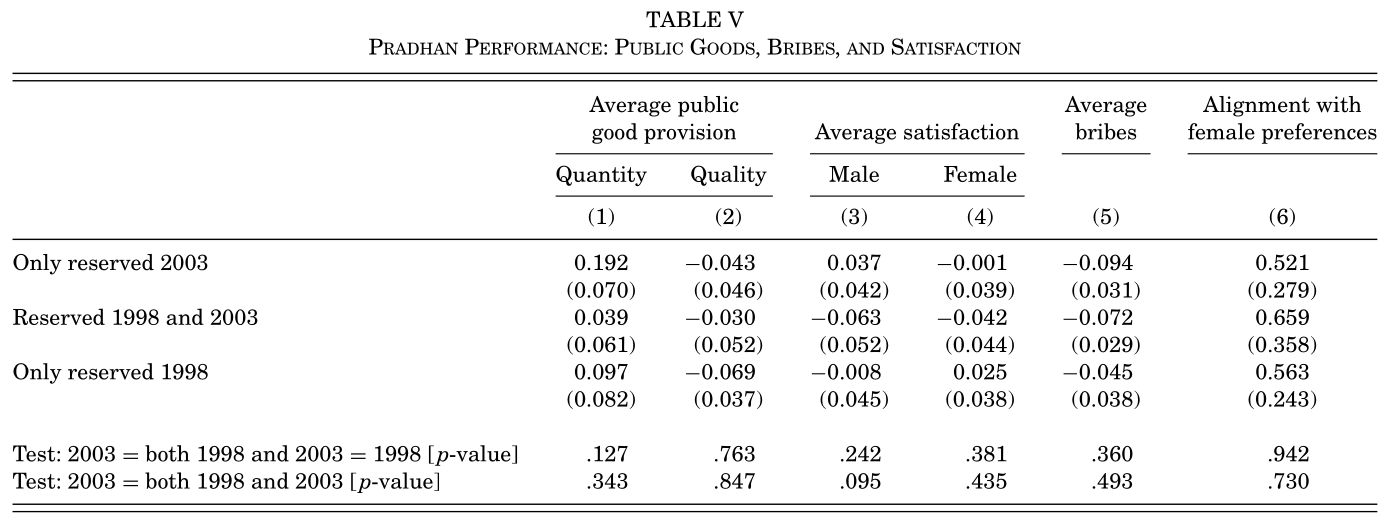
\includegraphics{20220523-qje-beaman-duflo-powerful-women.assets/table5-public goods performance.png}
\caption{Pradhan Performance: Public Goods, Bribes, and Satisfactions}
\end{figure}

\begin{itemize}
\tightlist
\item
  Performance and satisfaction was even greater for ``reserved 2003''

  \begin{itemize}
  \tightlist
  \item
    Not taking bribes: public opinion adversely influenced
  \item
    Aligned preference for women
  \end{itemize}
\end{itemize}
\end{frame}

\hypertarget{experiments-stereotypes-against-female}{%
\section{Experiments: Stereotypes Against
Female}\label{experiments-stereotypes-against-female}}

\begin{frame}{Experiment (1) Hypothetical Leader Effectiveness}
\protect\hypertarget{experiment-1-hypothetical-leader-effectiveness}{}
\begin{itemize}
\tightlist
\item
  Respondents were provided tape/vignette for policy speeches given by a
  pradhan
\item
  Same tape/vignette for each respondent, but substituting protagonist's
  gender to elicit implicit bias
\item
  Same questions regarding leader effectiveness
\end{itemize}
\end{frame}

\begin{frame}
\begin{figure}
\centering
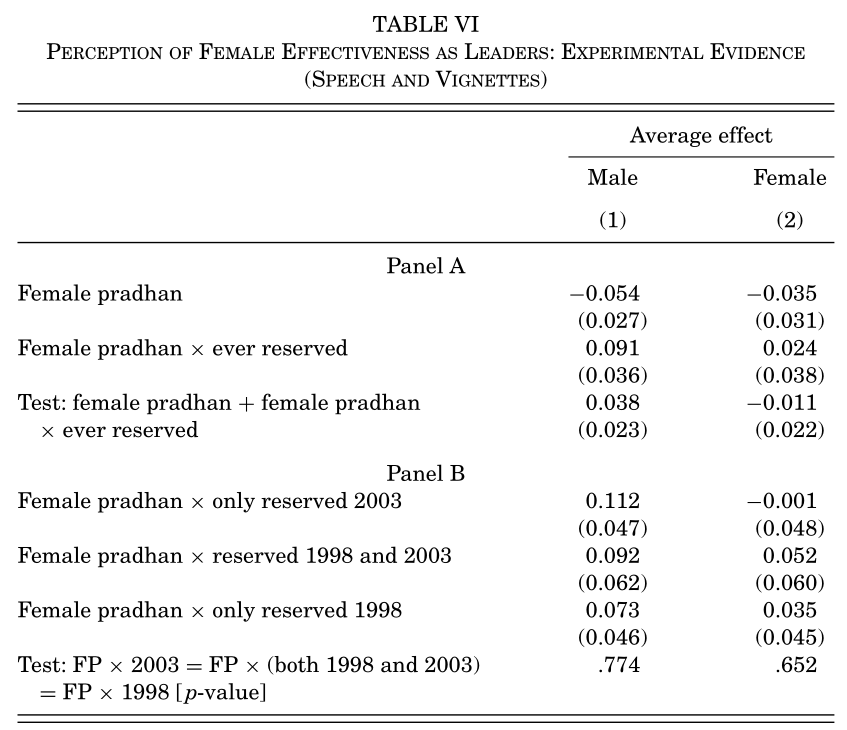
\includegraphics{20220523-qje-beaman-duflo-powerful-women.assets/table6-hypothetical effectiveness.png}
\caption{Perception of Hypothetical Leader Effectiveness}
\end{figure}

\begin{itemize}
\tightlist
\item
  Male's bias against female leader was updated after reservation
\item
  Female's belief wasn't updated: less involved in politics, or
  counter-stereotypic figure makes them feel uncomfortable
\end{itemize}
\end{frame}

\begin{frame}{Experiment (2) Implicit Bias of Gender}
\protect\hypertarget{experiment-2-implicit-bias-of-gender}{}
\begin{itemize}
\tightlist
\item
  IAT Experiment: Matching two concepts in short time
\end{itemize}

\begin{longtable}[]{@{}cc@{}}
\toprule
Left & Right \\
\midrule
\endhead
Male/Female Picture & Leadership/Domestic \\
Male/Female Name & Good/Bad \\
Male/Female Politician & Good/Bad \\
\bottomrule
\end{longtable}
\end{frame}

\begin{frame}
\begin{figure}
\centering
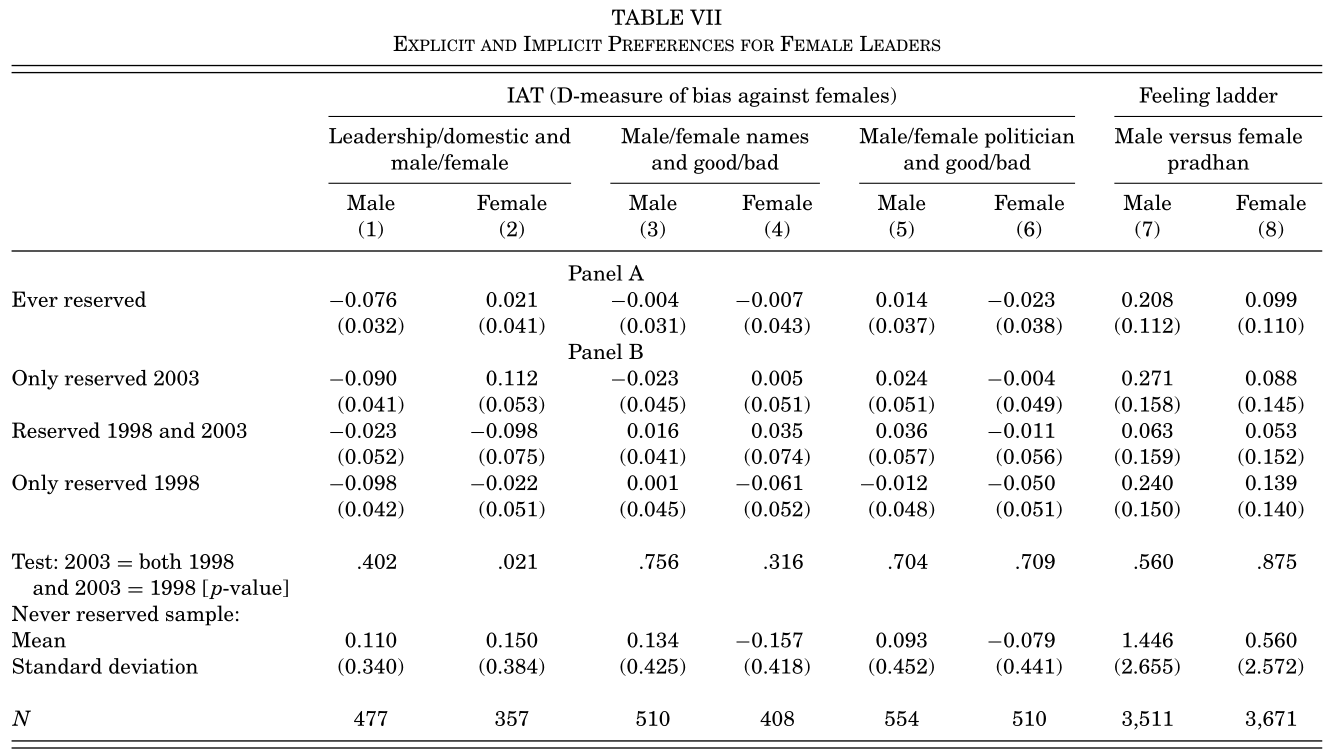
\includegraphics{20220523-qje-beaman-duflo-powerful-women.assets/table7-IAT results.png}
\caption{IAT Results and Feeling Ladder}
\end{figure}
\end{frame}

\hypertarget{conclusion}{%
\section{Conclusion}\label{conclusion}}

\begin{frame}{Conclusion}
\begin{itemize}
\tightlist
\item
  Gender quota helps improving female's political representation.
\item
  Gender quota reduced bias in evaluating female's political
  effectiveness, but some stereotypes persists.
\end{itemize}

\begin{block}{Related Subsequent Literatures}
\protect\hypertarget{related-subsequent-literatures}{}
\begin{itemize}
\tightlist
\item
  Female entrepreneurship \footnotesize (Ghani, Kerr, and O'Connell
  2014) \normalsize
\item
  Report of crimes against women \footnotesize (Iyer et al.~2012)
  \normalsize
\item
  Neonatal mortality of female \footnotesize (Kalsi 2017) \normalsize
\item
  Female educational attainment \footnotesize (Beaman et al.~2012)
  \normalsize
\end{itemize}
\end{block}

\begin{block}{}
\protect\hypertarget{section}{}
\end{block}
\end{frame}

\hypertarget{linkage-to-my-proposal}{%
\section{Linkage to My Proposal}\label{linkage-to-my-proposal}}

\begin{frame}{Contributions}
\protect\hypertarget{contributions}{}
\begin{itemize}
\tightlist
\item
  Taiwanese experience: Better IV consists of time and geographical
  variation
\item
  Further evidence on affirmative actions, public exposure of powerful
  women
\end{itemize}
\end{frame}

\begin{frame}{Current Findings}
\protect\hypertarget{current-findings}{}
\begin{itemize}
\tightlist
\item
  More female politician, less son preference.

  \begin{itemize}
  \tightlist
  \item
    Supported by both newborn data and survey data.
  \end{itemize}
\item
  Improved female's gender role self-recognition.
\end{itemize}
\end{frame}

\end{document}
